\documentclass[conference]{IEEEtran}

\usepackage{amsmath}
\usepackage{booktabs}
\usepackage{graphicx}
\usepackage{url}
\renewcommand{\UrlFont}{\rmfamily}

% TODO before submission: confirm the final author list with the supervisor.
% TODO before submission: the conference website gives conflicting instructions
% about double-blind review and author names; confirm whether anonymisation is required.

\title{Per-Class QoS Prediction and SLA Violation Detection for SD-WAN}

\author{\IEEEauthorblockN{Radhika (Rishiv) Shitlani}
\IEEEauthorblockA{School of Computer Science\\
University of Galway, Galway, Ireland}}

\begin{document}

\maketitle

\begin{abstract}
Software-defined wide area networks (SD-WANs) must treat traffic classes differently, yet a single strong overall accuracy score can mask poor performance for the class that most needs scrutiny: best-effort traffic. This paper predicts per-flow delay, detects service-level-agreement (SLA) violations, and predicts Bronze packet-loss risk, using 29,280 flow records from 400 BNNetSimulator runs covering Gold, Silver, and Bronze traffic under three scheduling policies and four scenarios. An XGBoost regressor evaluated with five-fold cross-validation reaches an overall log-delay $R^2$ of 0.766, with class-specific values of 0.914, 0.908, and 0.704 for Gold, Silver, and Bronze, and corresponding SLA-violation F1 scores of 0.944, 0.720, and 0.592. A multilayer perceptron and an FT-Transformer reach nearly identical scores on both delay regression and SLA detection. A paired exploratory comparison across the five folds detected no statistically significant XGBoost--MLP difference; given the small number of folds and their overlapping training data, this is treated as evidence that no clear performance advantage was observed, rather than proof that the models are statistically equivalent. The evaluation also shows that 90th-percentile delay is only moderately predictable, jitter is weakly predictable, and a binary Bronze packet-loss classifier reaches an AUC-ROC of 0.916. These results show that per-class, multi-metric evaluation is essential: a single global score hides both the gap between protected and best-effort traffic, and the boundary of what static configuration features can support.
\end{abstract}

\begin{IEEEkeywords}
SD-WAN, quality of service, machine learning, XGBoost, SLA prediction, per-class evaluation, packet loss
\end{IEEEkeywords}

\section{Introduction}

Software-defined wide area networking (SD-WAN) separates network control from packet forwarding, giving operators centralized control over routing and QoS policy across heterogeneous links. In practice, however, this control is typically exercised too late: operators adjust queue weights or reroute traffic only after congestion has already affected users. Predicting QoS ahead of an SLA breach could make this process proactive rather than reactive, but only if the prediction can be trusted for the traffic that most needs protecting. Gold, Silver, and Bronze traffic differ in priority, in how their delay behaves, and in what an error actually costs, so a model that appears accurate on average can still be unreliable for exactly the class most exposed to congestion.

Machine learning has already found several applications in SD-WAN research, including predicting how many virtual network functions a network will require~\cite{rahman2019autoscaling}, routing traffic based on application type~\cite{zheng2022applicationaware}, and steering traffic engineering with reinforcement learning~\cite{dinh2024safeloadbalancing,chen2025mteal}. Other work optimises SD-WAN routes and queueing policies directly from measured QoS~\cite{quang2022routing,quang2023globalqos}. These studies demonstrate that predictive or adaptive control is feasible, but none directly answer a narrower, more practical question: how accurately can continuous delay and SLA violations be predicted separately for each traffic class, and can Bronze packet-loss risk also be identified, from a compact and reproducible feature set?

This paper makes four contributions:
\begin{itemize}
    \item a reproducible per-class delay-prediction study using 29,280 flows from 400 BNNetSimulator runs, reporting regression and SLA-trigger performance separately for Gold, Silver, and Bronze traffic, and broken down further by scheduling policy and scenario;
    \item a comparison across three model families, XGBoost, a multilayer perceptron, and an FT-Transformer, on both delay regression and SLA detection, showing that additional model complexity does not improve per-class accuracy, supported by a paired statistical comparison that detected no significant difference;
    \item an extension of the evaluation to tail (90th-percentile) delay, jitter, and Bronze packet-loss risk, establishing the limits of what a static configuration feature set can support; and
    \item an SLA-threshold sensitivity analysis that quantifies the precision-recall trade-off used to select the operating threshold for best-effort traffic.
\end{itemize}

\section{Background}

SD-WAN replaces expensive, statically provisioned private circuits with software-based control over routing and QoS policy across heterogeneous links, such as broadband, LTE, and 5G, using edge devices, a central controller, and an overlay of logical tunnels over the physical underlay to enable dynamic path selection, fast failover, and traffic shaping.

QoS refers to the ability to give different priority levels to different traffic, and to guarantee a level of performance for the traffic that needs it most. The metrics of interest are latency, the time for a packet to travel from source to destination; jitter, the variation in that delay; packet loss; and available bandwidth. Delay-sensitive applications such as voice and video conferencing degrade quickly once these metrics fall outside an acceptable range, which is why SD-WAN operators write SLAs around them.

Machine learning is increasingly used to make QoS management proactive rather than reactive: forecasting traffic trends to adjust policy ahead of time, recommending routing paths from current and expected conditions, and predicting QoS metrics to warn of an SLA violation before it happens. This represents a shift from static, expert-tuned, one-size-fits-all configuration toward learned, class-aware, proactive decision support. This paper is concerned with the middle step of that pipeline: how accurately delay and SLA compliance can actually be predicted separately for each traffic class, and whether Bronze packet-loss risk can also be identified, before that prediction is used to drive a control decision.

\section{Related Work}

Machine learning has been applied to several adjacent network-management tasks, though rarely to per-class QoS prediction itself. Rahman \emph{et al.} use Random Forest and deep learning to predict how many virtual network functions a system will require as load changes, reporting over 95\% precision on the scaling decision itself, with the resulting proactive scaling used to reduce service degradation~\cite{rahman2019autoscaling}. Zheng \emph{et al.} combine supervised classification of traffic by application type with a QoS-aware routing algorithm that selects paths by delay tolerance~\cite{zheng2022applicationaware}. Both studies use machine learning to inform a decision rather than to predict a continuous QoS outcome per class, and neither reports class-wise prediction error.

Real-world suitability is a separate concern from raw accuracy. Dinh \emph{et al.} propose a deep reinforcement learning controller that maintains safe routing using control barrier functions~\cite{dinh2024safeloadbalancing}; GPU acceleration cuts their training time by roughly 110$\times$, though that practicality depends on GPU availability, which not every SD-WAN deployment has. Quang \emph{et al.} instead infer available link capacity from measurements the controller already collects, without probe traffic, using a model-based estimator (SABE) that feeds a two-loop routing-and-QoS controller and raised SLA satisfaction for critical traffic by roughly 40\% over static policies in their NS-3 evaluation~\cite{quang2023globalqos}. SABE is a strong non-learned baseline, but its queueing-theory assumptions do not describe the bursty, self-similar traffic of a real WAN, which is exactly the assumption a data-driven predictor could relax, and it motivates the learned approach taken here.

Integration into an operational system is a third concern. Quang \emph{et al.} describe a centralised SD-WAN controller that adjusts routing and scheduling from the current network state~\cite{quang2022routing}, reacting to the present rather than forecasting ahead of it, with no learned predictor involved. Rahman \emph{et al.} similarly show that scaling decisions triggered by a predictive model can reduce both QoS violations and cloud cost in a simulated scenario~\cite{rahman2019autoscaling}. Both confirm that automated decision support can be integrated into a live system, but neither predicts a QoS outcome per class ahead of time, which is the question this paper addresses.

Table~\ref{tab:lit-comparison} compares the reviewed literature against this paper. Across these works, a consistent pattern emerges: most rely on private or simulated traffic rather than a public, labelled SD-WAN QoS dataset; predict or optimise a single QoS dimension; do not treat Gold/Silver/Bronze classes explicitly, so class-level failures stay hidden behind a global metric; and do not compare deep learning against tree-based machine learning on the same task. Recent work also explores multi-objective, graph-based traffic engineering with reinforcement learning~\cite{chen2025mteal}. These gaps directly motivate the contributions listed above.

\begin{table*}[t]
\caption{Categorisation of Reviewed Literature Relative to This Paper}
\label{tab:lit-comparison}
\centering
\scriptsize
\setlength{\tabcolsep}{4pt}
\begin{tabular}{p{2.1cm}p{2.4cm}p{3.3cm}p{2.1cm}p{4.7cm}}
\toprule
Work & Technique & Main Focus & Data & Gap Relative to This Paper \\
\midrule
Rahman \emph{et al.}~\cite{rahman2019autoscaling} & RF + DNN & Predicting VNF requirements to maintain QoS and reduce cost & Private ISP traffic & VNF autoscaling only; no per-class QoS prediction \\
Zheng \emph{et al.}~\cite{zheng2022applicationaware} & Supervised ML + QoS routing & Classifying application types and assigning QoS-based routes & Constructed traffic + SDN sim. & Classification and routing; single metric, no class-wise error \\
Dinh \emph{et al.}~\cite{dinh2024safeloadbalancing} & DRL (PPO/DDPG) + CBF & Safe traffic routing respecting network constraints & Custom flow/packet sim. & Control-focused; heavy compute; no interpretable prediction \\
Quang \emph{et al.}~\cite{quang2023globalqos} & SABE (queueing) + local search & Estimating available bandwidth from passive measurements & NS-3 packet-level sim. & Model-based estimator and optimisation, not a learned predictor; no ML/DL comparison \\
Quang \emph{et al.}~\cite{quang2022routing} & Centralised optimisation & Managing QoS priorities and routing via SD-WAN controller & NS-3 packet-level sim. & Optimisation, not prediction; no ML model comparison \\
Chen \emph{et al.}~\cite{chen2025mteal} & GNN + MARL & SD-WAN traffic engineering with multi-dimensional QoS metrics & Public topology + sim. traffic & Complex control pipeline; not a reproducible per-class study \\
\textbf{This paper} & \textbf{XGBoost, MLP, FT-Transformer} & \textbf{Per-class delay, SLA violation, tail delay, jitter, and packet-loss risk prediction, with a tree-vs-deep-learning comparison} & \textbf{Reproducible simulator-generated data} & \textbf{Per-class, multi-metric QoS-aware evaluation with statistical significance testing} \\
\bottomrule
\end{tabular}
\end{table*}

When labelled enterprise telemetry is unavailable, network simulators offer a reproducible alternative. BNNetSimulator generates packet-level data compatible with the modelling methodology behind RouteNet-Fermi~\cite{bnnupc2023bnnetsimulator,ferriolgalmes2022routenetfermi}, and this study uses it to examine a narrower, more practical question than the wider literature addresses: can static configuration and path features alone support reliable, class-specific QoS prediction? XGBoost is used as the primary model because gradient-boosted trees remain strong performers on small-to-medium tabular datasets~\cite{grinsztajn2022trees,shwartzziv2022tabular}, train comparatively quickly, provide inexpensive split-based feature-importance measures, and support efficient Tree SHAP explanations.

\section{Methodology}

\subsection{Dataset and QoS Classes}

The dataset was generated with the official BNNetSimulator container~\cite{bnnupc2023bnnetsimulator} and contains 29,280 source-destination flow records from 400 simulation runs, with 30--132 flows per run. Traffic is divided into three classes: Gold (4,592 rows, highest priority), Silver (8,991 rows, interactive traffic), and Bronze (15,697 rows, best effort). The experiments span strict priority, WFQ, and deficit round robin scheduling across four scenarios: fixed WFQ weights, randomised WFQ profiles, and two mixed-policy scenarios with skewed and equal class proportions. The generator was configured to avoid deliberate near-saturation, so the results below should be read as a controlled study of per-class prediction rather than a stress test of a saturated production network.

Each input row includes the traffic class, offered bandwidth, traffic distribution, route length, network size, maximum average load, link bandwidth, scheduling policy, class queue weight, and minimum class weight. The prediction target is the natural logarithm of average delay in seconds. Any field that would leak the answer, namely raw delay, jitter, packet loss, delay percentiles, achieved bandwidth, the scenario label, and the simulation identifier itself, is excluded from the feature matrix. Missing numeric values are median-imputed and categorical variables are one-hot encoded, both computed separately within each training fold to avoid leakage.

\subsection{Prediction and Evaluation}

The primary regressor is XGBoost, configured with 200 trees, a maximum depth of four, a learning rate of 0.05, and row and feature subsampling both set to 0.9. Because the model is trained on log delay, predictions are converted back to milliseconds before being reported, so that the error values carry operational meaning. Performance is measured using mean absolute error (MAE) on the millisecond scale and $R^2$ on log delay.

Five-fold cross-validation is used, with folds constructed by randomly shuffling the full set of flow rows under a fixed random seed. Preprocessing and model fitting are refit independently within every fold, and every reported metric is derived from out-of-fold predictions rather than training predictions.

Continuous delay predictions are also converted into binary SLA-violation triggers. Gold and Silver use predefined experimental operating points of 30 and 50 ms, respectively. Bronze was initially assigned 100 ms, but an exploratory sensitivity sweep, reported in Section~\ref{sec:threshold}, led to a 60 ms operating point that improves recall while remaining more lenient than Silver. Precision indicates how much a trigger can be trusted once it fires, recall indicates how many real violations are actually caught, and F1 balances the two. None of these thresholds is a contractual SLA value drawn from a real deployment.

The same evaluation protocol and leakage-safe feature exclusions are reused for 90th-percentile delay and jitter. Bronze packet loss is treated separately as a binary risk-classification problem (whether a flow experiences any loss), using five-fold stratified cross-validation and class weighting to address the 89.3\%/10.7\% class imbalance.

\subsection{Reproducibility}

Data generation, preprocessing, evaluation, and plotting are implemented as separate, reusable Python scripts. Randomised estimators use a fixed seed (42), and every reported metric is derived from out-of-fold predictions rather than training predictions, ensuring that no result is inflated by the model having already seen the row it is scored on. The generated dataset, experiment scripts, and result tables are available in the project repository; a permanent archival identifier will be added for the camera-ready version.

\section{Results}

\subsection{Per-Class Delay and SLA Prediction}

Table~\ref{tab:main} reports the primary results. Overall $R^2$ is 0.766, with a delay-scale MAE of 12.63 ms, though this single figure conceals a substantial class-dependent gap. Gold and Silver are predicted accurately ($R^2=0.914$ and 0.908), while Bronze falls to 0.704 and its MAE grows by about 64\% to 20.68 ms. This pattern is consistent with protected traffic being shaped primarily by stable topology and scheduler configuration, which the static features capture well, while best-effort delay may also depend on transient contention that these features cannot observe.

\begin{table}[t]
\caption{Five-Fold Cross-Validation Results}
\label{tab:main}
\centering
\setlength{\tabcolsep}{3.5pt}
\begin{tabular}{lrrrrr}
\toprule
Class & MAE & $R^2$ & Prec. & Recall & F1 \\
 & (ms) & & & & \\
\midrule
Gold   & 3.05  & 0.914 & 0.994 & 0.899 & 0.944 \\
Silver & 3.48  & 0.908 & 0.823 & 0.639 & 0.720 \\
Bronze & 20.68 & 0.704 & 0.619 & 0.568 & 0.592 \\
\bottomrule
\end{tabular}
\end{table}

Gold's SLA trigger maintains a very high precision of 0.994: the model is correct 99.4\% of the time when it predicts a Gold violation. This is an important property for any controller that acts on such predictions, since false positives on the highest-priority class could trigger unnecessary intervention. Silver and Bronze are noticeably less reliable, particularly on recall, and Bronze's F1 of 0.592 illustrates an important point: a regressor that appears accurate in aggregate does not automatically translate into a strong SLA-violation detector for best-effort traffic.

\subsection{Scenario and Scheduling-Policy Analysis}

Table~\ref{tab:scenario} breaks the same XGBoost predictions down by simulation scenario. The mixed-policy scenario with skewed class proportions is the hardest to predict ($R^2=0.743$, MAE=21.32 ms), consistent with it combining strict priority, WFQ, and DRR scheduling within a single run and therefore presenting the model with the most heterogeneous queueing behaviour. The fixed-WFQ scenario is the easiest ($R^2=0.796$), since a single scheduling policy with a small, repeated set of weight values gives the model the most consistent structure to learn from.

\begin{table}[t]
\caption{Scenario-Specific Delay Prediction (XGBoost)}
\label{tab:scenario}
\centering
\setlength{\tabcolsep}{4pt}
\begin{tabular}{lrrr}
\toprule
Scenario & Rows & MAE (ms) & $R^2$ \\
\midrule
A (fixed WFQ)      & 6,560 & 6.16  & 0.796 \\
B (WFQ profiles)   & 8,240 & 12.01 & 0.758 \\
C (mixed, skewed)  & 7,600 & 21.32 & 0.743 \\
D (mixed, equal)   & 6,880 & 9.95  & 0.779 \\
\bottomrule
\end{tabular}
\end{table}

Table~\ref{tab:policy} slices the same predictions by scheduling policy instead of scenario. Strict priority (SP) reaches the highest $R^2$ (0.806) because SP flows follow a deterministic priority order that the model can learn directly. WFQ is harder ($R^2=0.756$) because its queue weights vary across profiles and interact with offered load in more complex ways. DRR shows the opposite pattern from what $R^2$ alone would suggest: it has the lowest absolute error (8.01 ms) but also the lowest $R^2$ (0.678), because $R^2$ measures variance explained within a class rather than the size of the error, and DRR's within-class delay variance is small enough that a modest absolute miss looks large in relative terms.

\begin{table}[t]
\caption{Scheduling-Policy Delay Prediction (XGBoost)}
\label{tab:policy}
\centering
\setlength{\tabcolsep}{4pt}
\begin{tabular}{lrrr}
\toprule
Policy & Rows & MAE (ms) & $R^2$ \\
\midrule
SP (strict priority)      & 8,120  & 8.27  & 0.806 \\
DRR (deficit round robin) & 1,840  & 8.01  & 0.678 \\
WFQ (weighted fair queue) & 19,320 & 14.90 & 0.756 \\
\bottomrule
\end{tabular}
\end{table}

\subsection{SLA Threshold Sensitivity}
\label{sec:threshold}

The Bronze SLA threshold used in Table~\ref{tab:main} (60 ms) was chosen after a sensitivity sweep rather than fixed in advance. Table~\ref{tab:bronze_sweep} shows how precision, recall, and F1 change as the threshold is lowered from an initial value of 100 ms. Lowering the threshold treats more flows as violations, which increases recall at some cost to precision; 60 ms was selected because it keeps Bronze strictly more lenient than Silver's 50 ms threshold while increasing recall by about 54\% relative to 100 ms, from 0.368 to 0.568, at a modest precision cost, from 0.726 to 0.619.

\begin{table}[t]
\caption{Bronze SLA Threshold Sensitivity}
\label{tab:bronze_sweep}
\centering
\setlength{\tabcolsep}{6pt}
\begin{tabular}{rrrr}
\toprule
Threshold & Precision & Recall & F1 \\
\midrule
100 ms & 0.726 & 0.368 & 0.488 \\
70 ms  & 0.614 & 0.476 & 0.536 \\
60 ms  & 0.619 & 0.568 & 0.592 \\
50 ms  & 0.582 & 0.735 & 0.650 \\
\bottomrule
\end{tabular}
\end{table}

A diagnostic Silver sweep shows the same precision-recall trade-off: at 32 ms, precision and recall reach 0.976 and 0.898, compared with 0.823 and 0.639 at the predefined 50 ms operating point. The 50 ms threshold is retained for consistency and is not presented as a contractual SLA.

\subsection{Model Complexity and Feature Evidence}

A comparison across model families, shown in Table~\ref{tab:models}, found nearly identical overall scores for XGBoost ($R^2=0.766$), a multilayer perceptron (0.766), and an FT-Transformer (0.762). All three model families reach essentially the same Bronze ceiling, and the FT-Transformer trails only marginally on Gold and Silver, with no gap exceeding 0.014 $R^2$. This is a signal that additional neural complexity provides little benefit here, since it cannot compensate for short-timescale traffic information absent from the feature set. XGBoost is retained as the model of choice for the remainder of the study because it matches the neural models while remaining interpretable and far less costly to train.

\begin{table}[t]
\caption{Per-Class Delay Prediction Across Models}
\label{tab:models}
\centering
\setlength{\tabcolsep}{4pt}
\begin{tabular}{lrrrr}
\toprule
Model & Overall & Gold & Silver & Bronze \\
 & $R^2$ & $R^2$ & $R^2$ & $R^2$ \\
\midrule
XGBoost        & 0.766 & 0.914 & 0.908 & 0.704 \\
MLP            & 0.766 & 0.912 & 0.908 & 0.705 \\
FT-Transformer & 0.762 & 0.900 & 0.898 & 0.703 \\
\bottomrule
\end{tabular}
\end{table}

SHAP values for the final XGBoost model support this conclusion (Fig.~\ref{fig:shap}). Route length dominates: additional hops push predictions toward higher log delay, while shorter paths pull them down. Network size and traffic class follow at some distance, with queue weights and scheduling-policy indicators contributing comparatively little on their own. These represent associations learned within the simulator rather than causal estimates, but they tell a consistent story: the model relies primarily on stable path structure. This structure is genuinely informative for protected Gold and Silver flows, but the weaker Bronze results suggest that it does not fully capture transient contention affecting best-effort delay.

\begin{figure}[t]
\centering
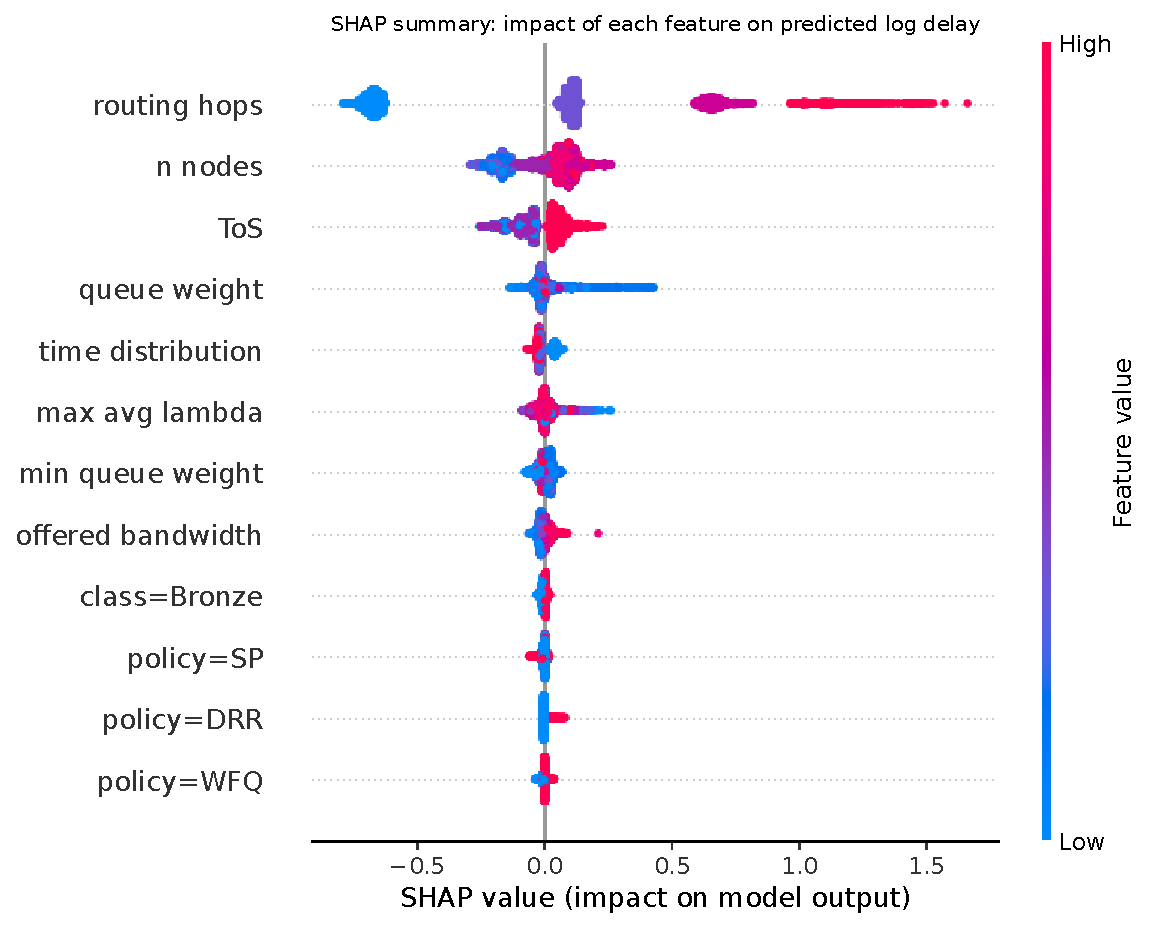
\includegraphics[width=0.95\columnwidth]{figures/shap_summary.pdf}
\caption{SHAP summary for the XGBoost log-delay model; colour denotes feature value.}
\label{fig:shap}
\end{figure}

\subsection{SLA Detection Across Models}

Table~\ref{tab:model_sla} compares SLA-violation detection across models at the selected experimental operating thresholds. Gold and Silver retain their predefined thresholds of 30 and 50 ms, while the Bronze threshold was selected as 60 ms following the sensitivity analysis in Section~\ref{sec:threshold}. The three models behave similarly, with only small differences in the precision-recall balance: the MLP leans slightly toward higher recall on the harder Silver and Bronze classes, while XGBoost and the FT-Transformer are marginally more precision-oriented. Gold precision stays very high across all three (0.98--0.99), which is the property that matters most for SD-WAN policy triggers, since a false positive on the highest-priority class would cause unnecessary rerouting.

\begin{table}[t]
\caption{SLA Detection Across Models at the Selected Experimental Thresholds}
\label{tab:model_sla}
\centering
\setlength{\tabcolsep}{3pt}
\begin{tabular}{llrrr}
\toprule
Class & Model & Prec. & Recall & F1 \\
\midrule
Gold   & XGBoost        & 0.994 & 0.899 & 0.944 \\
Gold   & MLP            & 0.979 & 0.908 & 0.942 \\
Gold   & FT-Transformer & 0.980 & 0.898 & 0.937 \\
Silver & XGBoost        & 0.823 & 0.639 & 0.720 \\
Silver & MLP            & 0.791 & 0.715 & 0.751 \\
Silver & FT-Transformer & 0.839 & 0.583 & 0.688 \\
Bronze & XGBoost        & 0.619 & 0.568 & 0.592 \\
Bronze & MLP            & 0.591 & 0.608 & 0.599 \\
Bronze & FT-Transformer & 0.597 & 0.580 & 0.589 \\
\bottomrule
\end{tabular}
\end{table}

\subsection{Statistical Significance of the XGBoost--MLP Difference}

The global difference between XGBoost and the MLP is small. Across the same five outer folds, the MLP is higher by a mean of 0.0006 $R^2$, while fold-to-fold variation is substantially larger. A paired $t$-test returns $p=0.620$, and a Wilcoxon signed-rank test returns $p=0.8125$. Neither test detects a statistically significant difference at the 0.05 level.

These results do not prove that the models are equivalent: a formal equivalence test would require a predefined margin representing the smallest practically meaningful difference. In addition, cross-validation fold estimates are not fully independent because their training sets overlap. The appropriate conclusion is therefore that this experiment found no measurable advantage for either model, consistent with their nearly identical observed scores.

\subsection{Tail Delay and Jitter}

Table~\ref{tab:secondary} applies the same evaluation to two secondary QoS targets. Tail delay is noticeably harder to predict than average delay: Gold and Silver reach only moderate $R^2$ values of 0.635 and 0.657, and Bronze falls much further to 0.258, with its MAE climbing to 38.22 ms. This is expected, since the 90th percentile captures rarer, more variable congestion events than the mean, and the same gap that separates Bronze from Gold and Silver on average delay is amplified in the tail.

Jitter is very weakly predicted across every class, with $R^2$ ranging only from 0.014 (Bronze) to 0.119 (Gold). This is a meaningful finding rather than a modelling failure: the feature set describes static network configuration, such as queue weights, scheduling policy, and offered bandwidth, and these features determine mean delay well but do not capture the moment-to-moment traffic burstiness that drives jitter.

\begin{table}[t]
\caption{Per-Class Results for Secondary QoS Targets}
\label{tab:secondary}
\centering
\setlength{\tabcolsep}{5pt}
\begin{tabular}{llrr}
\toprule
Target & Class & MAE (ms) & $R^2$ \\
\midrule
Delay p90 & Gold    & 6.64  & 0.635 \\
          & Silver  & 7.29  & 0.657 \\
          & Bronze  & 38.22 & 0.258 \\
\midrule
Jitter    & Gold    & 0.14 & 0.119 \\
          & Silver  & 0.16 & 0.084 \\
          & Bronze  & 3.11 & 0.014 \\
\bottomrule
\end{tabular}
\end{table}

\subsection{Bronze Packet Loss}

Non-zero packet loss is concentrated primarily in Bronze traffic. Gold and Silver record only 4 and 93 loss events respectively across 13,583 combined flows, whereas 1,684 of 15,697 Bronze flows (10.7\%) experience some loss. This distribution is consistent with the simulator configuration protecting higher-priority traffic, although it should not be interpreted as validation against a real production network.

Because the operational question is whether a Bronze flow is at risk of experiencing loss, packet loss is evaluated as a binary classification problem, using class weighting (\emph{scale\_pos\_weight}=8.3) to address the 89.3\%/10.7\% class imbalance. Table~\ref{tab:bronze_loss} reports five-fold stratified cross-validation results.

\begin{table}[t]
\caption{Bronze Binary Loss Classification}
\label{tab:bronze_loss}
\centering
\setlength{\tabcolsep}{4pt}
\begin{tabular}{lrrrr}
\toprule
Model & Prec. & Recall & F1 & AUC-ROC \\
\midrule
XGBoost (default)        & 0.777 & 0.328 & 0.461 & 0.914 \\
XGBoost (class-weighted) & 0.342 & 0.865 & 0.490 & 0.916 \\
Random Forest (balanced) & 0.663 & 0.389 & 0.490 & 0.895 \\
\bottomrule
\end{tabular}
\end{table}

The class-weighted XGBoost classifier reaches an AUC-ROC of 0.916, indicating strong ranking ability. At the default 0.5 decision threshold, class weighting raises recall to 0.865 but reduces precision to 0.342, meaning roughly two of every three flagged flows do not actually experience loss; a false-alert rate this high risks alert fatigue, where operators or downstream automation begin to distrust the system's warnings. The appropriate operating threshold therefore depends on the relative cost of a missed loss event against a false alarm, and should be set deliberately, for example from a precision-recall curve, rather than by a default cut-off.

\section{Discussion and Limitations}

The central finding here is not simply that delay is predictable, but that its predictability depends heavily on the traffic class and on which target is being predicted. Route length, network size, and traffic class encode stable structure, and this structure explains protected average delay well: the SHAP analysis shows route length dominates by a wide margin, exactly the kind of static, configuration-level quantity the model has access to. Bronze has the lowest configured class priority or weight. Under strict-priority scheduling it is served after Gold and Silver, whereas WFQ and DRR share service among classes according to their configured weights or quanta. Its delay can therefore depend on transient queue contention and short traffic bursts that the current features do not measure. The same limitation helps explain why Bronze tail delay is harder still: the tail is precisely where contention events can dominate.

The three model families reach very similar observed performance, and the exploratory paired comparison detects no significant XGBoost--MLP difference. This is consistent with the possibility that the available features constrain performance more strongly than model capacity, although the present experiment does not prove that explanation or establish formal model equivalence.

The weak jitter results and the packet-loss classification trade-off suggest that the static feature set does not fully capture the short-timescale conditions affecting these outcomes. Dynamic measurements such as recent queue occupancy, arrival-rate windows, inter-arrival statistics, and recent loss may improve their prediction. This remains a hypothesis for future experiments rather than a causal conclusion established by the present results.

Several limitations should temper these claims. First, no real-world enterprise SD-WAN dataset with labelled QoS metrics was available for this work, so the results rely on data generated by BNNetSimulator rather than measured on a live network. The evaluation measures performance on held-out flow records generated by BNNetSimulator; it does not establish transfer to a real enterprise SD-WAN. Second, the feature set is entirely static: telemetry such as instantaneous queue occupancy, recent arrival-rate windows, and recent loss would be required to model transient behaviour, and none of this is present here. Third, all SLA thresholds used are experimental operating points rather than contractual values drawn from a real deployment. Future work should add dynamic traffic features to improve Bronze delay, tail delay, jitter, and packet-loss prediction, and should validate the approach against real controller telemetry.

\section{Conclusion}

This paper presented a per-class, multi-metric evaluation of QoS prediction for SD-WAN-like networks. XGBoost predicts Gold and Silver average delay accurately but is less reliable for Bronze, tail delay, and jitter. A binary Bronze packet-loss classifier remains strongly discriminative, although its precision-recall balance depends substantially on the selected operating point. XGBoost, the MLP, and the FT-Transformer achieve similar observed performance: the paired fold comparison detects no statistically significant XGBoost--MLP difference, so the experiment provides no evidence that additional neural complexity improves this task, though this should not be interpreted as a formal demonstration of model equivalence. The scenario and scheduling-policy breakdown further shows that prediction performance varies with the simulated operating conditions, from the deterministic ordering of strict priority to the more heterogeneous mixed-policy scenarios. The broader implication is straightforward: trustworthy AI-assisted QoS prediction requires class-aware, multi-metric evaluation, and an honest account of what static network features can and cannot support.

\bibliographystyle{IEEEtran}
\bibliography{references}

\end{document}
